\section{Introduction}
Edge intrusion detection must balance attack recognition with latency and energy. Runtime selection appears attractive, but a learned controller may simply choose one detector throughout deployment. Comparing it only with a more expensive static detector then measures an operating-point change rather than adaptive value. In our primary campaign, Tabular-Q saves 13.1 J over roughly 500 s relative to Static-MedRF---1.08\%, or 26.1 mW on average---while missed-positive presentations rise from 57.8 to 565.9 per 50,000-row replay. This scale mismatch motivates a stricter question: \emph{what schedule was actually realized, under what service constraints, and at what security cost?}

We answer that question as a \ton{}-centered systems study with four frozen detectors and paired Raspberry Pi measurements; \cic{} and \nb{} remain supplementary detector/data audits rather than dynamic-power evidence. The evidence separates the primary physical campaign and Static-LightLR attribution control, an analytic reward non-degeneracy screen, and prospectively frozen confidence/deadline-aware controls under fixed and variable load.

Four questions organize the paper: \emph{RQ1}, what security/resource operating points do the frozen \ton{} detectors provide? \emph{RQ2}, do learned selectors improve upon the static schedule they realize, and is their scalar objective non-degenerate on the declared support? \emph{RQ3}, do confidence- and deadline-aware conditional controls provide useful switching? \emph{RQ4}, how do state coverage, off-support actions, deadline violations, and threshold calibration constrain deployment claims?

Our contributions are: (i) paired whole-device evidence that places a small resource effect beside its much larger missed-detection cost; (ii) a pairwise non-degeneracy criterion that converts reward weights and normalization into a pre-deployment preference-reversal test; (iii) static, learned, confidence-cascade, and variable-load controls that separate detector choice from conditional orchestration; and (iv) an off-support failure analysis showing how sparse discrete-state coverage can expose unsafe default actions. Together, the study identifies when learned IDS orchestration does---and does not---realize adaptive service value.

\begin{figure*}[t]
\centering
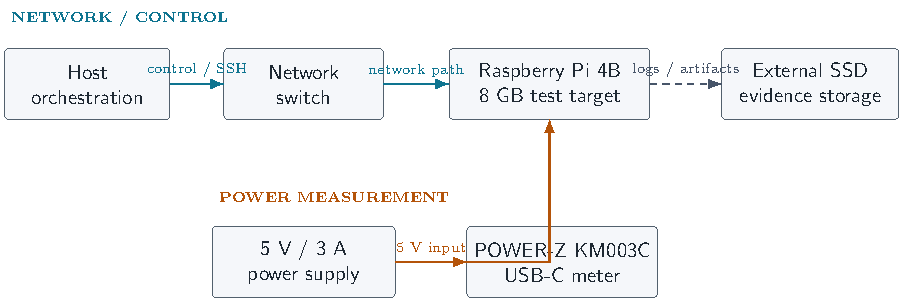
\includegraphics[width=.82\textwidth]{figures/experiment_setup_schematic.pdf}
\caption{Schematic apparatus overview. Network orchestration reaches the Raspberry Pi 4B through the switch, while the 5-V supply feeds the Pi through the KM003C meter; the external SSD stores evidence artifacts. The drawing identifies roles and paths only and contains no synthetic measurement readout.}
\label{fig:experimentdesign}
\end{figure*}
